\subsection{Parameter Estimation for ARMA processes}

When fitting parameter estimates to a realization of an ARMA(1,1) model, we can leverage a transformed version of the likelihood equation based on the one step predictors $\hat{X}_{t+1} = \mathbb{E}(X_{t+1}|X_t,X_{t-1},...,X_1)$.

Let $\Sigma_X$ be the $T \times T$ covariance matrix of the zero-mean ARMA(1,1) Gaussian process $\{X_t\}$. The likelihood equation is then given by:

$$L(\phi,\theta,\sigma^2|\mathbf{X}) = (2\pi)^{-T/2}|\Sigma_X|\text{exp}\left\{\mathbf{X}'\Sigma_X^{-1}\mathbf{X}\right\}$$ 

From Brockwell and Davis \cite{BrockwellDavis1991}, we can rewrite this likelihood as follows:

$$ L(\phi,\theta,\sigma^2|\mathbf{X}) = (2\pi\sigma^2)^{-T/2}(r_0 - \cdots r_{T-1})^{-1/2}\text{exp}\left\{ -\frac{1}{2\sigma^2}\sum_{j=1}^T\frac{(X_j - \hat{X}_j)^2}{r_{j-1}} \right\}$$

The one step predictors $\{\hat{X}_t\}_{t=1}^T$ and their corresponding mean squared errors $\{r_t = \sigma^{-2}\mathbb{E}(X_{t+1} - \hat{X}_{t+1})^2\}_{t=0}^{T-1}$ are given by the Innovations Algorithm:


\begin{equation}
    \label{eq:innovations_r_theta}
    \begin{cases}
    \hat{X}_1 = 0 \\
    r_0 = \sigma^{-2}\gamma_X(0) = 1 + \frac{(\phi + \theta)^2}{(1 - \phi^2)} \\
    \theta_{t1}= \theta / r_{n-1}\\
        \hat{X}_{t+1} = \phi X_t + \theta_{n1}(X_t - \hat{X}_t) \\
    r_t = 1 + \theta^2 - \theta^2/r_{t-1}, & t \geq 1 
\end{cases}
\end{equation}



This recursive sequence of coefficients can be initially inaccessible, but we see in Figure \ref{fig:innovations_r_theta} that $\theta_{t1}$ and $r_t$ both rapidly approach $\theta$ and 1, and their respective values for small values of $t$ account for the lack of history at the start of the time series.

\begin{figure}
    \centering
    \begin{subfigure}{.45\textwidth}
    \centering
    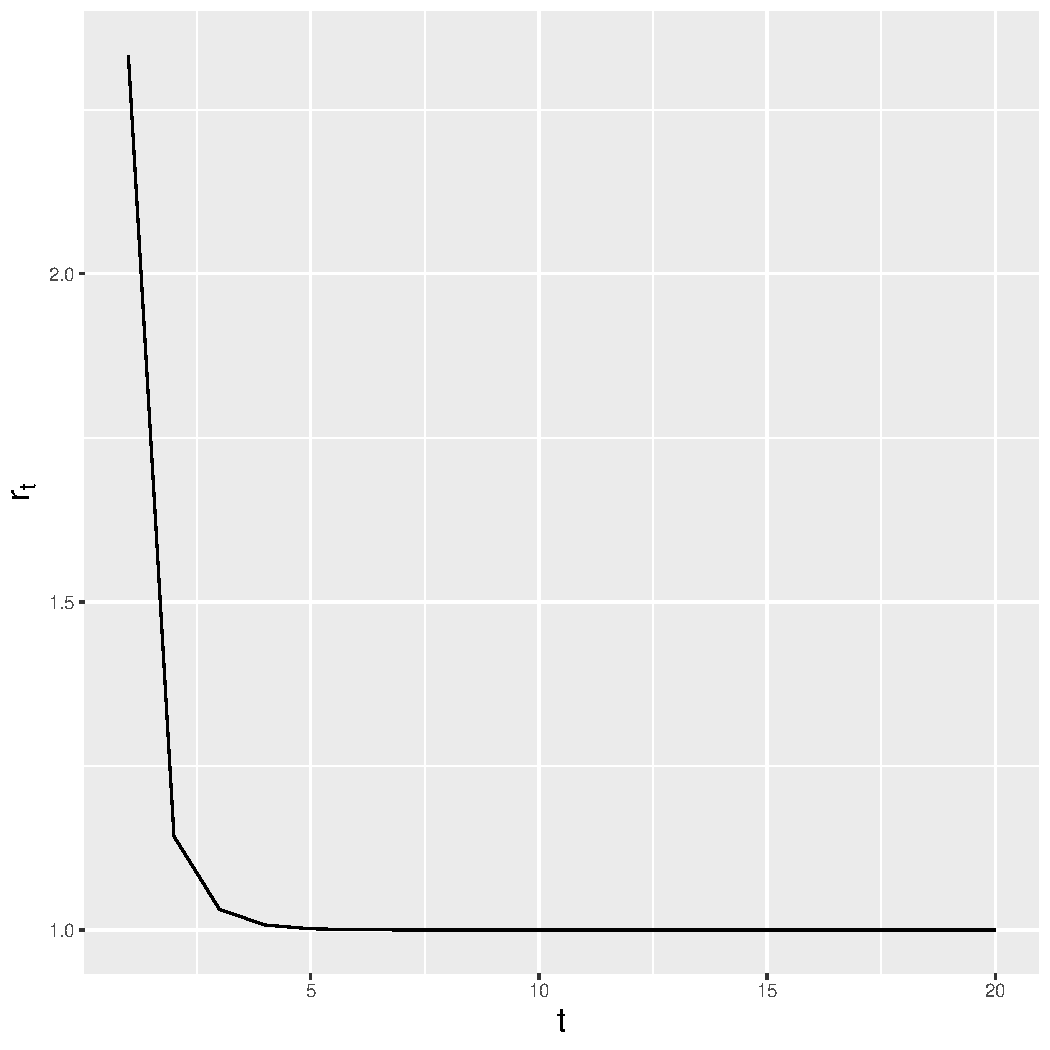
\includegraphics[width=\textwidth]{images/output/r_t.pdf}
    \caption{Values of $r_{t-1}$}
  \end{subfigure}
    \hfill
    \begin{subfigure}{0.45\textwidth}
        \centering
        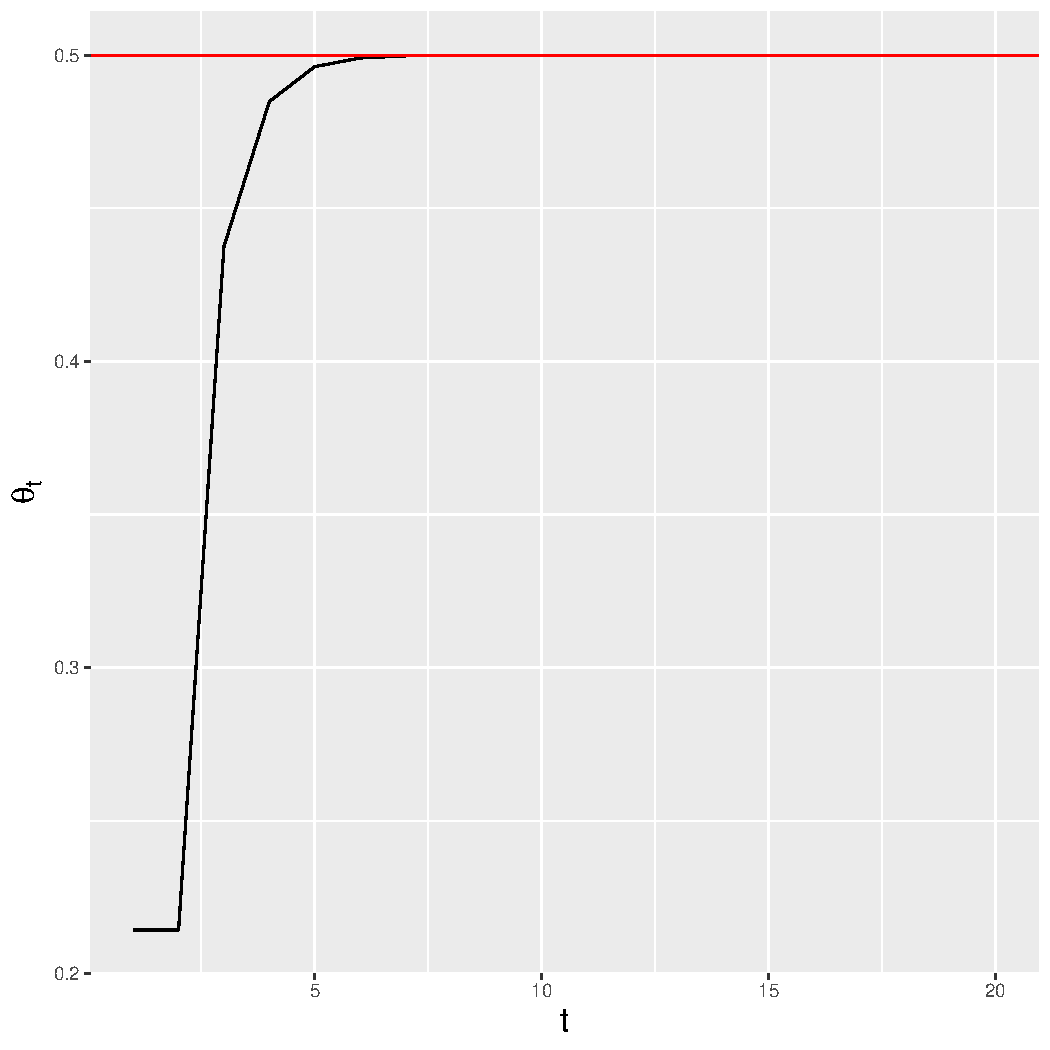
\includegraphics[width=\linewidth]{images/output/theta_t1.pdf}
        \caption{Values of $\theta_{t1}$}
    \end{subfigure}
    \caption{Coefficients provided by Innovations Algorithm for Calculating One-Step Predictors of ARMA(1,1) process}
    \label{fig:innovations_r_theta}
\end{figure}

It doesn't take long for the one step predictors detailed in Equation \ref{eq:innovations_r_theta} to be effectively equivalent to $\hat{X}_{t+1} = \phi X_t + \theta(X_t - \hat{X}_t)$ with $\mathbb{E}(X_t-\hat{X}_t)^2 = \sigma^2$. We now derive the MLE for $\sigma^2$ using this new expression of the likelihood:

\begin{equation}
    \label{eq:logLik_innov}
    l(\phi,\theta, \sigma^2) = -\frac{T}{2}\text{ln}(2\pi\sigma^2)-\frac{1}{2}\text{ln}\left(\prod_{t=1}^Tr_{t-1}\right) - \frac{1}{2\sigma^2}\sum_{t=1}^T\frac{(X_t - \hat{X}_t)^2}{r_{t-1}}
\end{equation}

$$ l(\phi,\theta, \sigma^2) = -\frac{T}{2}\text{ln}(2\pi\sigma^2)-\frac{1}{2}\sum_{t=1}^T\text{ln}(r_{t-1}) - \frac{1}{2\sigma^2}\sum_{t=1}^T\frac{(X_t - \hat{X}_t)^2}{r_{t-1}} $$

Noting that $\{r_t\}$, $\{\theta_{t1}\}$ and consequently $\{\hat{X}_t\}$ are all functions independent of $\sigma^2$, we obtain the following derivative:

$$ \frac{\partial }{\partial \sigma^2}l(\phi,\theta, \sigma^2) = -\frac{T}{2\sigma^2} + \frac{1}{2\sigma^4}\sum_{t=1}^T\frac{(X_t - \hat{X}_t)^2}{r_{t-1}} \equiv 0$$
Defining $S(\phi,\theta):= \frac{\sum_{t=1}^T(X_t - \hat{X}_t)^2}{r_{t-1}}$, we know $\hat{\sigma}_{\text{ML}}^2$ must satisfy:

$$ \hat{\sigma}^2_\text{ML} = \frac{S(\hat{\phi},\hat{\theta})}{T} $$
Substituting this back into our log likelihood, we obtain:

$$ l(\phi,\theta, \sigma^2) = -\frac{T}{2}\text{ln}(2\pi) - \frac{T}{2}\text{ln}(T^{-1}S(\phi,\theta))-\frac{1}{2}\sum_{t=1}^T\text{ln}(r_{t-1}) - \frac{T}{2S(\phi,\theta)}S(\phi,\theta) $$

$$ l(\phi,\theta, \sigma^2) = -\frac{T}{2}\left[\text{ln}(2\pi) +\text{ln}(T^{-1}S(\phi,\theta))+\frac{1}{2}\sum_{t=1}^T\text{ln}(r_{t-1}) + \frac{1}{S(\phi,\theta)}S(\phi,\theta)\right] $$

By removing the constant terms we can deduce that $\hat{\phi}$ and $\hat{\theta}$ must minimize the expression: 

$$ \text{ln}(T^{-1}S(\phi,\theta))+\frac{1}{2}\sum_{t=1}^T\text{ln}(r_{t-1})$$

Doing so is a numerical process that is greatly facilitated by good initial estimates, which can be calculated with such methods as the Durbin-Levinson Algorithm, the Innovations Algorithm, and/or the Yule-Walker Algorithm depending on the order of the time series \citep{BrockwellDavis1991}. The asymptotic behavior of the Maximum Likelihood Estimator and its implications on inference are discussed in the next section.





 











% We can re-express this equation for $p = q =1 $ using the backwards operator $B$:

% $$ (1-\phi B)X_t = (1 + \theta B)Z_t $$



% Because we are imposing that the time series is causal, we have:

% $$ X_t = \sum_{j=0}^\infty \psi_jZ_{t-j} $$

% We therefore can express $\gamma_X(h)$ as:

% $$ \gamma_X(h) = \sigma^2\sum_{j=0}^\infty \psi_j\psi_{j+|h|} $$

% Because $\psi(B):= \sum_{j=0}^\infty\psi_jB^j = \theta(B)/\phi(B) $, we can produce a system of equations by equating coefficients of $B^j$:

% $$ \phi (B) \psi (B) = \theta(B) $$

% For our restricted $p=q=1$ case, this reduces to:

% $$ (1-\phi B)\sum_{j=0}^\infty \psi_j B^j = (1 + \theta B), $$

% and the resulting system is:

% $$ \begin{cases}
%     \psi_0 = 1 \\
%     \psi_1 - \phi \psi_0 = \theta \\
%     \psi_2 - \phi\psi_1 = 0 \\
%     \psi_3 - \phi \psi_2 = 0 \\
%     \hspace{.25in}\vdots
% \end{cases} $$

% From this we get the following successive set of equations for $\{\psi_j\}$
% $$ \begin{cases}
%     \psi_0 = 1 \\
%     \psi_1 = \phi + \theta \\
%     \psi_2  =  \phi(\phi + \theta)  \\
%     \psi_3 = \phi^2 (\phi + \theta) = 0 \\
%     \hspace{.25in}\vdots
% \end{cases} $$

% Now because we have two parameters $(\phi,\theta)$ to estimate , we will need a system of two equations, and thereby require estimates for $\psi_1$ and $\psi_2$. From the above system of equations it is clear that with these estimates $\hat{\psi}_1, \hat{\psi}_2$ we can solve for $\phi$ and $\theta$. All that remains is to actually find said estimates. We use the following estimates:

% $$ \begin{cases}
%     \hat{\psi}_1 = \hat{\theta}_{21} \\
%     \hat{\psi}_2 = \hat{\theta}_{22},
% \end{cases} $$

% where $\hat{\theta}_{21}, \hat{\theta}_{22}$ are given by the Innovations Algorithm \citep{BrockwellDavis1991} (Definition 8.3.1), and given explicitly below:
% $$ \begin{cases}
%     \hat{\nu}_0 = \hat{\gamma}(0) \\
%      \hat{\theta}_{11} =  \hat{\nu}_0^{-1}\left[ \hat{\gamma}(1) \right] \\
%      \hat{\nu}_1 = \hat{\gamma}(0) - \hat{\theta}_{11}^2 \hat{\nu}_0 \\
%      \hat{\theta}_{22} = \hat{\nu}_0^{-1}\left[\hat{\gamma}(2) \right] \\
%      \hat{\theta}_{21} = \hat{\nu}_1^{-1}\left[ \hat{\gamma}(1) - \hat{\theta}_{22}\hat{\theta}_{11}\hat{\nu}_0 \right] \\
%      \hat{\nu}_2 = \hat{\gamma}(0) - \hat{\theta}_{22}^2\hat{\nu}_0 - \hat{\theta}_{21}^2\hat{\nu}_1
% \end{cases} $$





% Estimates for $\psi_1,..., \psi_{p+q}$ are obtained using estimates $\hat{\theta}_{m1},...,\hat{\theta}_{m,p+q}$ from the Innovations Algorithm (See Appendix). Replacing $\psi_j$ with $\hat{\theta}_{mj}$ in the equation above we obtain:

% $$ \hat{\theta}_{mj} = \theta_j + \sum_{i=1}^{\text{min}(j,p)} \phi_i \hat{\theta}_{m,j-i}, \qquad j = 1,2,...,p + q $$

% This reduces in the $p=q=1$ case to\textcolor{blue}{Check $\hat{\theta}_{20} = 1$}:


% $$ \begin{cases}
%     \hat{\theta}_{21} = \theta + \phi \\
%     \hat{\theta}_{22} = \phi 
% \end{cases} $$

% We can then solve for $\hat{\bm{\phi}}$ using the equation:

% \begin{equation}
%     \left[ \begin{array}{c}
%          \hat{\theta}_{m,q+1}  \\
%           \hat{\theta}_{m,q+2} \\
%           \vdots \\
%           \hat{\theta}_{m,q+p}
%     \end{array} \right] = \left[ \begin{array}{cccc}
%         \hat{\theta}_{m,q} & \hat{\theta}_{m,q-1} & \cdots & \hat{\theta}_{m,q+1-p} \\
%         \hat{\theta}_{m,q+1} &\hat{\theta}_{m,q} & \cdots & \hat{\theta}_{m,q+2-p} \\
%          \vdots& \vdots & & \vdots \\
%          \hat{\theta}_{m,q+p-1}& \hat{\theta}_{m,q+p-2} & \cdots & \hat{\theta}_{m,q}
%     \end{array} \right] \left[ \begin{array}{c}
%          \phi_1 \\
%          \phi_2 \\
%          \vdots \\
%          \phi_p
          
%     \end{array} \right]
% \end{equation}

% In the $p = q = 1$ case this reduces to:
% \begin{equation}
%          \hat{\theta}_{2,2} /     \hat{\theta}_{2,1}  =:          \hat{\phi} 
% \end{equation}

% After solving this system, $\hat{\bm{\theta}}$ is found from:

% $$ \hat{\theta} = \hat{\theta}_{mj} - \sum_{i=1}^{\text{min}(j,p)}\hat{\phi}_i\hat{\theta}_{m,j-i}, \qquad j = 1,2,...,q,  $$

% which reduces to:

% $$ \hat{\theta}_{21} - \hat{\phi} $$


% Once these steps are complete, innovation variance can be estimated with $\widehat{\sigma^2} = \hat{v}_2$. Pre-compiled R packages like \emph{arima} can be used to fit these models, and are able to handle missing time steps that tend to occur in repeated survey settings. Let's now look at the asymptotic distributions of these estimators for the purposes of inference.